% REPLACE: "recall" instead of "factual" knowledge questions
% INTRO: motivate process/structure NOT content

% OUTLINE INTRO %
% 1. Assessing political competence is important, but the measurement debate remains unresolved
% 2. Factual knowledge questions are insufficient, we should focus on what people know and not what they don't know
% 3. This is where my measure comes in, describe basic idea and contribution
% 4. Outline of the paper and describe basic findings + conclusion

Political sophistication is one of the most fundamental concepts in the study of political attitudes and behavior. While scholars have long emphasized people's alarmingly low levels of sophistication \citep{converse1964nature,carpini1996americans}, fundamental issues regarding its measurement continue to plague the discipline \citep[e.g.,][]{mondak2001developing,sturgis2008experiment}. Scholars usually rely on survey questions that assess individuals' ability to recall basic facts about political institutions and officeholders as a proxy for sophistication \citep[e.g.,][]{zaller1990political,carpini1993measuring}. In principle, these factual knowledge questions should cover information that is necessary and/or sufficient for citizens to make competent decisions in a given context \citep{lupia2006elitism}, but determining such a set of items proves to be extremely difficult---especially since there are systematic differences in types of knowledge \citep{barabas2014question}. Even within a given policy area, people may disagree about which facts are crucial for political competence due to inherent value differences \citep{lupia2015uninformed}. Furthermore, to the extent that items vary in difficulty across subgroups (i.e., differential item functioning), relying on standard knowledge batteries may introduce systematic measurement error \citep{pietryka2013analysis}.

One manifestation of such systematic measurement error is the oft-cited gender gap in sophistication. On the basis of conventional factual knowledge scores, women frequently appear to be less informed about politics than men \citep{verba1997knowing,wolak2011roots}. However, some scholars suggest that these differences might an artifact of the measurement approach. For instance, \citet{mondak2004knowledge} argue that at least part of the gender gap can be attributed to the fact that women are less likely to guess than men when facing a factual knowledge question for which they do not know an immediate answer. Others argue that the gap can be attenuated by focusing on gender-relevant political knowledge \citet[e.g.,][]{dolan2011women} or by providing policy-specific information \citep[e.g.,][]{jerit2017revisiting}.

In this paper, I re-examine the gender gap by proposing a measure of \textit{discursive sophistication} that is based on how people discuss their political preferences in open-ended survey responses. Specifically, I develop a framework to assess whether beliefs and attitudes in a given political domain are expressed in a more elaborate manner---a question that is not directly discernible from off-the-shelf factual knowledge items. %The approach is therefore \textit{naive} in that it does not presuppose pieces of information as necessary for political competence but rather examines the respondents' justification of their preferences at face value. 
Measuring sophistication based on how people talk about politics provides two major advantages compared to off-the-shelf factual knowledge items: (1) it captures the extent to which a respondent's political beliefs are based on elaborate reasoning, and (2) it can easily pinpoint competence in specific areas by incorporating targeted open-ended items and (3) it is conceptually closer to the degree of structure and constraint in political belief systems \citep[see for example][]{tetlock1983cognitive,luskin1987measuring}.

I validate the measure across multiple data sets by comparing it to conventional factual knowledge scores as predictors of various indicators of civic competence and engagement. However, while the measures share a considerable amount of variance, they are far from equivalent. Indeed, discursive sophistication is a stronger predictor of turnout and other forms of political participation than traditional metrics. Contrary to previous research, however, I find no evidence for such a gap in discursive sophistication. While women might score lower than men on factual knowledge about political institutions and elites, there are no differences in the complexity of expressed political attitudes. This divergence can be explained by the fact that open-ended responses allow women to focus on different issues than men. More generally, the results suggest that measuring political sophistication based on open-ended responses can provide new opportunities to examine political knowledge across time and contexts.


\section*{Political Sophistication and Factual Knowledge}

In his seminal study on political attitudes, \citet{converse1964nature} examined whether citizens hold constrained belief systems about politics. Belief systems are defined as ``a configuration of ideas and attitudes in which the elements are bound together by some form of constraint or functional interdependence'' \citep[207]{converse1964nature}. The majority of the electorate, it turns out, does not hold structured and constrained belief systems, understand abstract ideological concepts, or hold stable issue positions. This pessimistic view regarding the competence of the U.S. electorate has been supported in multiple subsequent analyses. \citet{carpini1996americans} show that large parts of the American electorate are not sufficiently informed about politics and that there are systematic differences in political attitudes and behavior between citizens who are well informed compared to those who are not. These findings are problematic from a normative perspective, since they indicate that differences in political information can result in unequal representation in the political system \citep[see also][]{althaus1998information,kuklinski2000misinformation,gilens2001political}. However, rather than relying on the degree to which individuals possess constrained belief systems, \citet{carpini1996americans} conceptualized knowledge as the awareness of key democratic values, using factual knowledge questions \citep[see also][]{carpini1993measuring}. Many studies focus on similar factual knowledge measures \citep[e.g.,][]{zaller1991information,gomez2001political}. For example, \citet{zaller1992nature} measures political awareness using tests of neutral factual information about politics, since they ``more directly than any of the alternative measures, capture what has actually gotten into peoples minds'' \citep[21]{zaller1992nature}. However, other research casts doubt on this assertion, both from methodological as well as theoretical perspectives.

From a methodological perspective, many studies raised issues related to the validity of factual knowledge questions as a measure of political sophistication. One problem are potential biases due to guessing \citep{mondak2000reconsidering,mondak2001asked,miller2008experimenting}. Responses to knowledge items that offer a ``Don't Know'' option are simultaneously influenced individual information levels as well as the propensity to guess. Other scholars further criticized open-ended factual knowledge questions due to problematic coding rules, which do not capture partial knowledge \citep{krosnick2008problems,gibson2009knowing,debell2013harder}.

Focusing solely on factual political knowledge has also been criticized on theoretical grounds. \citet{lupia2006elitism} argues that the information asked for has no clear relevance to political participation. Instead, researchers should concentrate on heuristics that directly help citizens to make competent political decisions or focus only on knowledge relevant to a specific task \citep[see also][]{lupia1994shortcuts}. Accordingly, there is no need for individuals to know all available facts, but only to possess the skills and resources to be able to find the information required in a specific context \citep{prior2008money}. Furthermore, conventional items differ with regard to the dimension of political knowledge they measure \citep{barabas2014question} and ignore important aspects such as visual cues \citep{prior2014visual}.


\section*{Please Mind the Gender Gap}

A common finding in public opinion research is that women have lower levels of observed political knowledge than men. For example, \citet{verba1997knowing} report that women score lower on political information, interest, and efficacy, which decreases their respective levels of political participation. Since gender differences in political information and interest can only partly be explained by resource-related factors such as individual levels of education, the authors diagnose a ``genuine difference in the taste for politics'' between women and men, which they suspect is driven largely by socialization \citep[see also][]{wolak2011roots}. Indeed, \citet[117]{dow2009gender} describes the systematic gender differences in knowledge as ``one of the most robust findings in the study of political behavior.'' Other scholars, however, argue that the disparities between women and men may simply be an artifact of the measurement approach.

The discussion revolving around the apparent gender gap is therefore closely intertwined with the methodological debate about measuring political knowledge. For instance, \citet{mondak2004knowledge} suggest that women are more likely to report that they do not know the answer to a recall question whereas men are more inclined to guess. Correcting for the systematic differences in the propensity to guess, however, mitigates the gender gap in knowledge but does not eliminate it completely \citep[see also][]{lizotte2009explaining}. Other aspects of the survey context have been shown to affect gender differences in political knowledge as well. \citet{mcglone2006stereotype}, for example, present evidence that the gender gap is exacerbated in an environment that induces stereotype threat, such as if women are aware of the fact that the study focuses on gender differences or if they are interviewed by a male interviewer. However, gender differences are not only induced by \textit{how} researchers ask their questions, but also by the question \textit{content}, since focusing on gender-relevant political knowledge items such as information about women's representation in the federal government has been shown to close the gap \citep{graber2001processing,dolan2011women,fraile2014does,jerit2017revisiting}. Similarly, \citet{stolle2010women} report that the gender gap disappears when people are asked about more practical issues related to the government (e.g., benefits and services).

Overall, the gender gap has been shown to be influenced by how we ask for political information in surveys, as well as the kind of knowledge that is required for a correct response. Indeed, a comprehensive cross-national analysis of election studies in 47 countries between 1996 and 2011 suggests that question format and content account for large portions of the variance of gender disparities in political knowledge \citep{fortin2016cross}.


\section*{Back to the Roots: The Structure of Belief Systems}
% Attitude Expression and Elaborate Reasoning
% Conceptualizing Discursive Sophistication

% OUTLINE MEASUREMENT %
% 1. How can we characterize in-depth processing in open-ended responses? We don't want to look at textual complexity, as other recent research has done.
% 2. It's about the speaker, not the recipient! This is were the literature on belief systems comes in! Theoretical accounts of political sophistication as the basis for elaborate and in-depth political reasoning
% 3. Derive the three dimensions conceptually, connect them to belief system literature -> survey example!
% 4.-6. Now we discuss how we can measure them in open-ended responses

% How can we characterize the level of sophistication in open-ended responses that engage in more in-dpeth processing? This is where the literature on belief systems comes in.
% Next, I will explore specific attributes that allow us to distinguish more or less elaborate reasoning in open-ended responses.
% If we To the extent that people's political sophistication and competence manifests itself in attitude expression 
% Recent studies in political science, for example, used measures based on the readability or comprehensibility to study the sophistication of political communication
% measuring the degree of elaborate reasoning in verbatim attitude expression

Many conventional item batteries to assess political sophistication have problematic measurement properties, which may exacerbate observed gender differences. Rather than trying to develop a new item battery that addresses some of these issues, I propose an alternative approach. Instead of testing respondents on a specific set of predetermined facts, we can make inferences about political sophistication by analyzing how they discuss their attitudes and beliefs in their own words. As described above, \citet{converse1964nature} explicitly conceptualized political sophistication based on the level of constraint in political beliefs rather than isolated pieces of factual information. Similarly, \citet{tetlock1983cognitive} used the term integrative complexity to describe the degree to which considerations related to an issue are interconnected.

From a theoretical perspective, political sophistication therefore characterizes a particular \textit{structure} of an individual's system of beliefs about politics. For example, \citet{converse1964nature} emphasizes the importance of the level of conceptualization as the main characteristic of sophistication rather than isolated pieces of factual information. Similarly, \citet{tetlock1983cognitive,tetlock1993cognitive} uses the term \textsl{integrative complexity} to describe the degree to which considerations related to an issue are interconnected. \citet{luskin1987measuring} also defines political sophistication based on the structure of individual belief systems, arguing that they can vary on three separate dimensions: (1) their \textsl{size} -- i.e. the number of cognitions, (2) their \textsl{range} -- i.e. the dispersion of cognition over categories, and (3) their \textsl{constraint} -- i.e. the extent to which cognitions are interconnected in a meaningful way. Political sophistication, in turn, is seen as the conjunction of these dimensions: ``A person is politically sophisticated to the extent to which his or her [political belief system] is large, wide-ranging, and highly constrained'' \citep[860]{luskin1987measuring}. Sophisticated political reasoning should reflect this notion of complex belief systems.\footnote{It should be no surprise that Converse and others examined open-ended responses in their early studies--albeit from a slightly different perspective than the approach outlined here. Importantly, instead of relying on manual coding of open-ended responses, I develop an automated framework that is easily reproducible and can directly be applied to large surveys.}

First, let us examine response variation across survey items. Individuals who engage in elaborate processing should hold opinions about each political actor or policy they are asked to discuss. Given a set of multiple open-ended probes focusing on different targets of evaluation, sophisticated respondents should be able to express their attitudes towards each question more or less equally.% in terms of both approval or disapproval.

% 1) Distribution between answers
\begin{proposition}[Size] % Considerations, Depth
Political sophistication is characterized by a belief system that encompasses a large number of considerations.
\end{proposition}

Next, the level of elaboration should also be related to the content and topics raised by each individual. Respondents who possess a large and wide-ranging belief system should be able to discuss their views from multiple perspectives rather than focusing only on a single consideration.

% 2) Distribution across topics/considerations
\begin{proposition}[Range] % Opinionation, Breadth
Political sophistication is characterized by a belief system that includes a wide ranges of categories.
\end{proposition}

Lastly, we can examine variation in the way each consideration itself is being talked about, particularly focusing on individual differences in word choice. Sophisticated respondents should use terms that are highly descriptive of a given topic---for example by mentioning interest rates or unemployment when talking about economic policies.
% rather than broad terms that could be attributed to any topic and are not clearly related to politics.

% 3) Distribution within topics
\begin{proposition}[Constraint] % Word Choice, cognitive complexity, Integration
Sophisticated respondents are aware of key concepts related to an issue and therefore use terms that are clearly associated with a given topic.
\end{proposition}

% Discursive sophistication in attitude expression is then defined as the conjunction of these three basic dimensions.
In a questionnaire where respondents are asked to discuss their political attitudes in multiple open-ended items, I therefore define discursive sophistication as the conjunction of the three dimensions described here. Overall, a highly sophisticated individual can be expected to give a more elaborate response to every question that focuses on multiple considerations using terms that are highly descriptive of each topic. Note that this simple framework makes no strong assumptions about the type of information necessary to make competent decisions in a given context; neither does it make assumptions about whether a given argument is correct or not. Crucially, since it is solely based on \textit{how} individuals discuss their preferences, it can be directly applied in various settings to target specific political tasks such as choosing between candidates, parties, or policy propositions. Rather than having to devise a new set of questions that attempt to capture information necessary to make competent decisions, we can simply analyze how respondents describe and justify their political preferences in verbatim.
% In the following, I discuss these three different attributes of open-ended survey responses that should be indicative of sophistication in attitude expression in more detail.

Of course, this is not the first time a framework is developed to assess the complexity of written (or spoken) word. In fact, this task has been the subject of longstanding research in linguistics and educational sciences, resulting in a multitude of alternative metrics. Recently, these measures have been employed by political scientists who study different forms of elite communication. \citet{spirling2016democratization}, for example, uses a standard readability score based on the ratio of words per sentence and syllables per word to study the linguistic complexity of speeches in the British House of Commons over time. More recently, \citet{benoit2019measuring} expanded on previous metrics to develop a measure of comprehensibility that is more applicable in the realm of politics.
% \citet{spirling2016democratization}: The findings reveal that ministers started to use simple language in the parliament after suffrage was expanded in the middle nineteenth century---presumably in an effort to appeal to the enlarged voter base. 

These approaches---and especially the development of metrics specifically suited for political text---are particularly useful when studying elite communication. Yet, in contrast to the framework outlined above, they focus on the \textit{comprehensibility} as a measure of complexity; sophistication is evaluated based on a recipient's ease to understand the message, which is largely driven by linguistic and syntactic difficulty rather than actual political content. Again, while this is certainly a reasonable approach when studying the effects of elite communication, the inference of interest outlined in this paper is markedly different. My focus is to examine verbatim attitude expression to assess the underlying degree of elaborate political reasoning. Pure linguistic style is therefore not of central concern so long as it is unrelated to the actual political content.\footnote{In fact, one might be concerned that pure linguistic complexity is ultimately driven by other factors such as a person's general verbosity or linguistic prowess and therefore not a valid measure of political sophistication.} After all, being hard to comprehend does not necessarily imply that someone put a lot of thought into a statement.
% Reading level measures essentially focus on how hard it is to understand the author. This makes sense if we are primarily interested in the messaging aspect, for example when analyzing speeches of political elites. When it comes to individual levels of sophistication, a pure focus on linguistic patterns are less ideal.
% However, while these techniques are certainly useful to examine complexity in messaging by political elites, they may be highly confounded by personal verbosity and linguistic prowess. Instead of assessing linguistic style, we want to target the complexity in the actual content. Rather than measuring how a specific attitude is delivered, we want to focus on the the complexity in what is being said.
% The inference of interest is not how easy it is to understand someone, but rather how much thought went into what has been said. Both are clearly correlated, but they should not be assumed to be equivalent.
% comprehensibility of the text captures more of the linguistic ability independent of the underlying political content.


\section*{Measuring Discursive Sophistication}
% A First Look at Discursive Sophistication

In the following, I propose a framework that leverages the content of open-ended responses in conjunction with the survey structure to evaluate the underlying reasoning that gives rise to individual statements. Consider for example a questionnaire where respondents are prompted to describe their attitudes toward major presidential candidates and their parties in multiple open-ended items. Each question asks for either positive or negative considerations related to one of the parties or candidates. In developing a measure of political sophistication, we are ultimately interested in people's level of elaboration when justifying their preferences in such a set of open-ended responses. So how would a politically sophisticated person who engages in in-depth processing discuss her views compared to a less informed individual?

Consider again the example of multiple open-ended questions regarding candidate and party preferences in a survey. In such a scenario, we can characterize elaborate reasoning by leveraging variation in response patterns on three levels---across questions, between topics mentioned, and within each topic. For each dimension, I make the following assumptions regarding the way sophistication manifests itself in verbatim responses.

In order to measure discursive sophistication according to the theoretical framework outlined above, we need to quantify individual-level variation in open-ended responses on each of the three dimensions. I begin by describing the measurement approach in more detail and explore a first set of results based on data from the 2012 and 2016 ANES. The same procedures are applied to the remaining datasets and additional information for these is provided in the appendix.

Sophisticated respondents evaluate political actors and issues on multiple dimensions and are therefore able to recall a large number of distinct considerations in response to each query presented in a survey.

The first component targets the \textit{size} of the belief system by measuring the number of considerations discussed by each individual. I rely on the structural topic model framework to extract the number of topics mentioned by each respondent in a survey \citep{roberts2014structural}.\footnote{Please refer to the appendix for additional information. Specifically, see Appendix~\ref{app:oeinfo} for descriptive information on open-ended responses in each dataset and structural topic model results. Appendix~\ref{app:topicmodel} contains further details on pre-processing steps and modeling choices for the structural topic models as well as robustness checks, which include preText analyses proposed by \citet{denny2018text}.} I denote $\mathcal{W}_i$ as the set of words contained in a response of individual $i$. Each word $w\in\mathcal{W}_i$ is assigned to a topic $t^* \in \{1,...,T\} $, such that $P(t^*|w,X_i) > P(t|w,X_i) \forall t\neq t^*$.\footnote{Note that $P(t|w,X_i)=\tfrac{P(w|t)P(t|X_i)}{P(w|X_i)}$. In the context of structural topic models, $X_i$ denotes the covariates used to predict individual topic prevalence \citep[see][for details]{roberts2014structural}. I used measures for age, gender, education, party identification, as well as an interaction between education and party identification as covariates for topic prevalence. This variable selection---with the exception of including gender---is equivalent to the procedure described in \citet{roberts2014structural}.} In other words, each unique term in a response is assigned to the topic that has the highest likelihood of having generated that term, given the model. The set of topics that are mentioned by respondent $i$ across all words in $\mathcal{W}_i$ can then be described as $\mathcal{T}^*_i$ and the number of considerations can be written as:
\begin{equation}
\text{size}_i = \dfrac{|\mathcal{T}^*_i|}{\max|\mathcal{T}^*_i|}.
\end{equation}
I re-scale the measure to range from zero to one by dividing raw count of topics by the maximum number of topics observed across individuals.

Second, regarding response patterns across questions, high levels of elaboration have been argued to display a greater \textit{range}, which is based on the degree to which individuals are able to respond to each query presented in a survey more or less equally. I quantify this diversity in relative lengths for each open-ended response as the Shannon entropy across survey items:
\begin{equation}
\text{range}_i = \dfrac{-\sum_{j=1}^J p_{ij} \ln p_{ij}}{\ln J}
\end{equation}
where $p_{ij}$ is the proportion of words in the response of individual $i$ to question $j\in \{1,...,J\}$ relative to the overall size of the individuals' response. The variable ranges from 0 (only one question was answered) to 1 (all questions were answered with the same word length per answer).

The last component of discursive sophistication addresses the way individuals talk about each consideration. More specifically, I argue that when discussing a specific topic, sophisticated respondents should use words that are clearly associated with it since they are aware of relevant key concepts. We can again rely on the structural topic model result to summarize the extent to which \textit{word choice} consists of highly descriptive terms for each topic, which implies that a specific term has a high likelihood to be mentioned if a given topic is discussed. Thus, highly descriptive word choice is conceptualized as the sum of term likelihoods $P(w|t^*)$ given topic assignments over the entire set of words in $\mathcal{W}_i$:
\begin{equation}
\text{constraint}_i = \dfrac{\sum_{\mathcal{W}_i} P(w|t^*)}{\max\left[\sum_{\mathcal{W}_i} P(w|t^*)\right]}
\end{equation}
As before, I re-scale the measure to range from zero to one by dividing all values by the empirical maximum observed across all individuals in the data.


\section*{A First Look at Discursive Sophistication}

Applying this approach to both waves of the ANES shows that all three components are highly correlated.\footnote{See Appendix~\ref{app:oeinfo} for correlation matrices between individual components for the ANES as well as the remaining two datasets.} Furthermore, an exploratory factor analysis confirms that all three components load on a single factor with all loadings exceeding 0.5. Detailed results are presented in Table~\ref{app:factload}.

% latex table generated in R 4.2.1 by xtable 1.8-4 package
% Wed Aug 10 12:57:08 2022
\begin{table}[ht]
\centering
\begin{tabular}{lcccc}
  \hline
Variable & 2018 CES & 2020 ANES & 2016 ANES & 2012 ANES \\ 
  \hline
Size & 0.840 & 0.997 & 0.997 & 0.997 \\ 
  Range & 0.526 & 0.536 & 0.548 & 0.576 \\ 
  Constraint & 0.513 & 0.684 & 0.623 & 0.709 \\ 
   \hline
\end{tabular}
\caption{Factor Loadings of Discursive Sophistication Components} 
\label{app:factload}
\end{table}


Together, the three measures can therefore be combined in a composite metric of sophistication in political attitude expression by averaging them for each respondent. Like each individual component, the resulting \textit{discursive sophistication} score ranges from 0 to 1:
\begin{equation}
\text{discursive sophistication}_i = \tfrac{1}{3}(\text{opinionation}_i + \text{considerations}_i + \text{word choice}_i).
\end{equation}

We can now compare discursive sophistication to alternative metrics of political knowledge. As discussed in the beginning, the standard approach to measuring political knowledge in surveys is to ask a set of factual questions about political institutions. The ANES surveys include such a basic item battery, inquiring for example about the number of times an individual can be elected President of the United States, or how the current U.S. federal budget deficit compares to the deficit in the 1990s. I combine responses on these items to form an additive index of \textit{factual knowledge} about politics. As an additional benchmark, I consider \textit{interviewer assessments} of each respondent's political sophistication (see \citealt{bartels2005homer} for an example of a study that relies on interviewer assessments; but cf. \citealt{ryan2011accuracy}).\footnote{Interviewer assessments were only recorded in the face-to-face sample of the ANES.}

\begin{figure*}[h]
    \centering
    \begin{subfigure}[t]{0.45\textwidth}
    	\centering
    	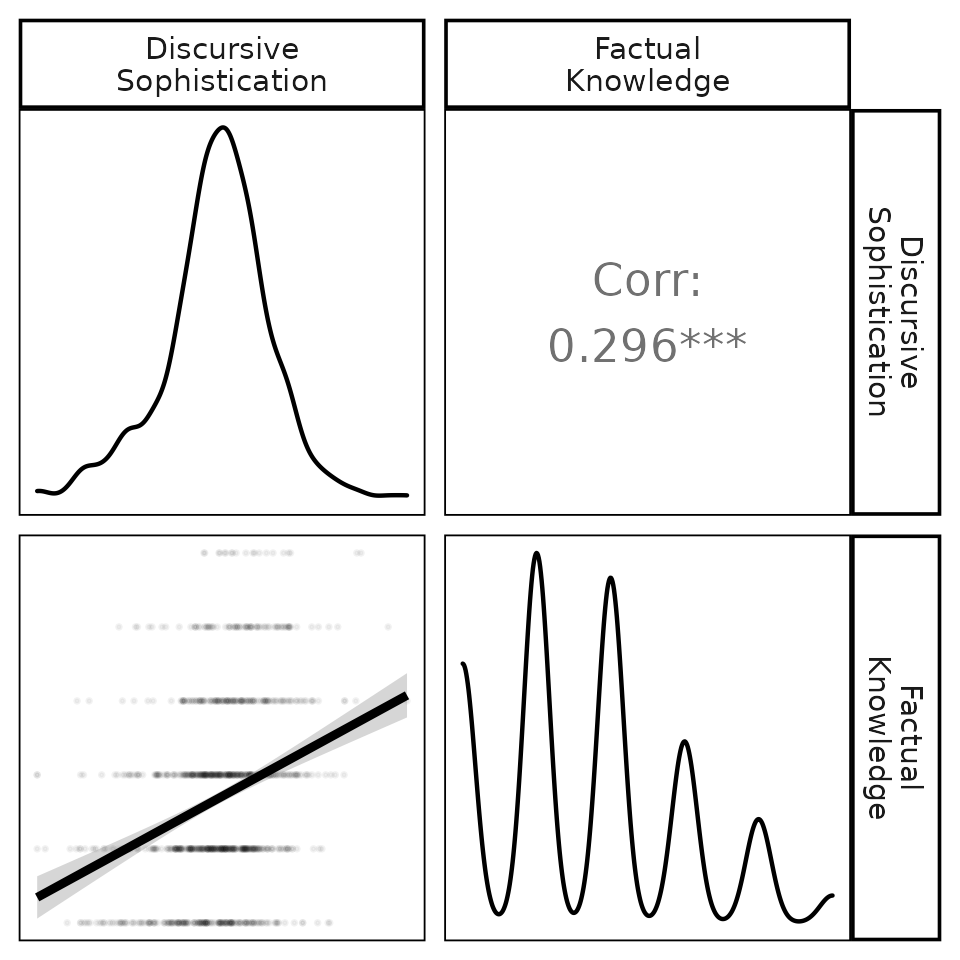
\includegraphics{/data/Dropbox/Uni/projects/2016/knowledge/fig/cces2018_corplot.png}
    	\caption{2018 CES}
    \end{subfigure}
	~~
    \begin{subfigure}[t]{0.45\textwidth}
    	\centering
    	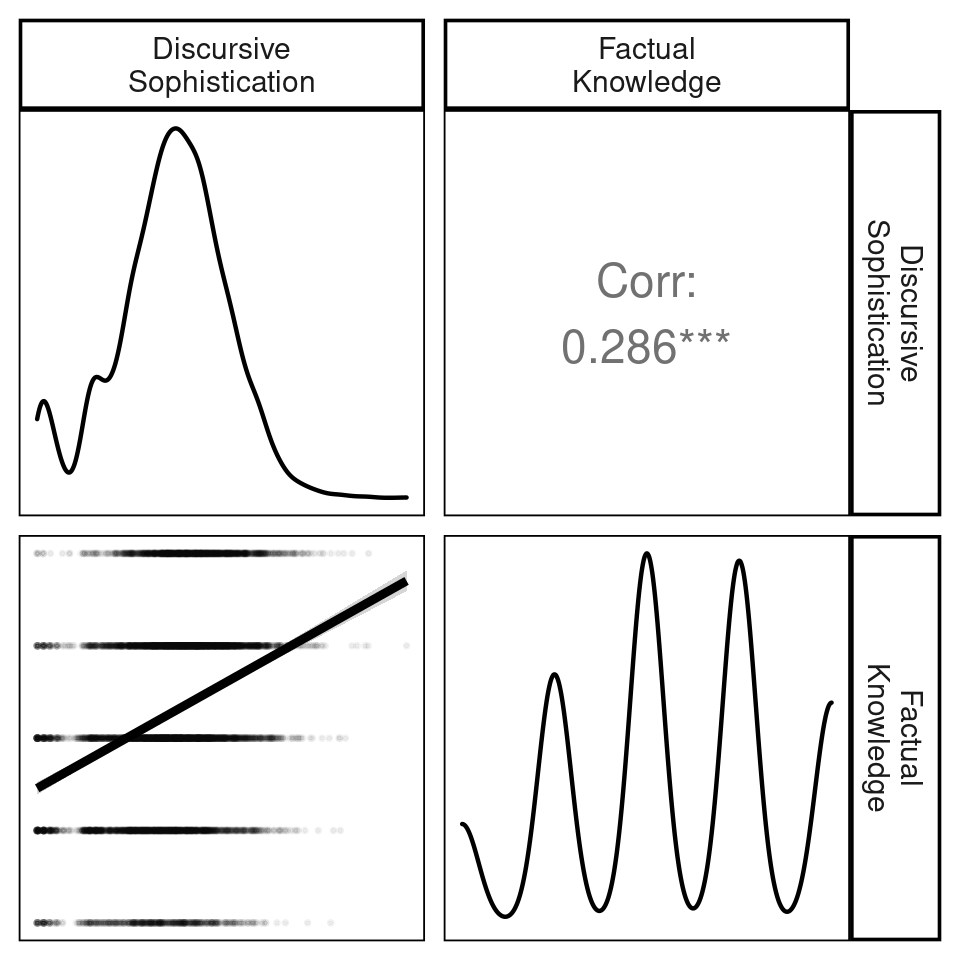
\includegraphics{/data/Dropbox/Uni/projects/2016/knowledge/fig/anes2020_corplot.png}
    	\caption{2020 ANES}
    \end{subfigure}
    \begin{subfigure}[t]{0.45\textwidth}
    	\centering
    	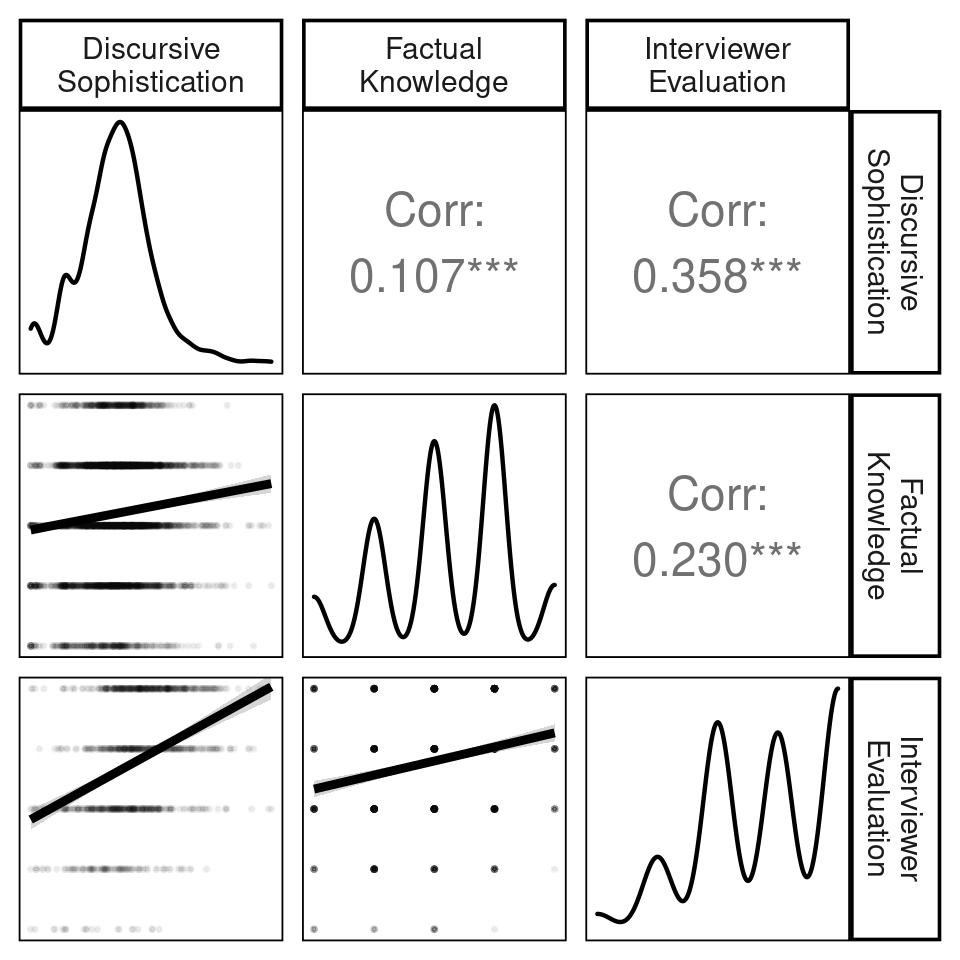
\includegraphics{/data/Dropbox/Uni/projects/2016/knowledge/fig/anes2016_corplot.png}
    	\caption{2016 ANES}
    \end{subfigure}
	~~
    \begin{subfigure}[t]{0.45\textwidth}
        \centering
        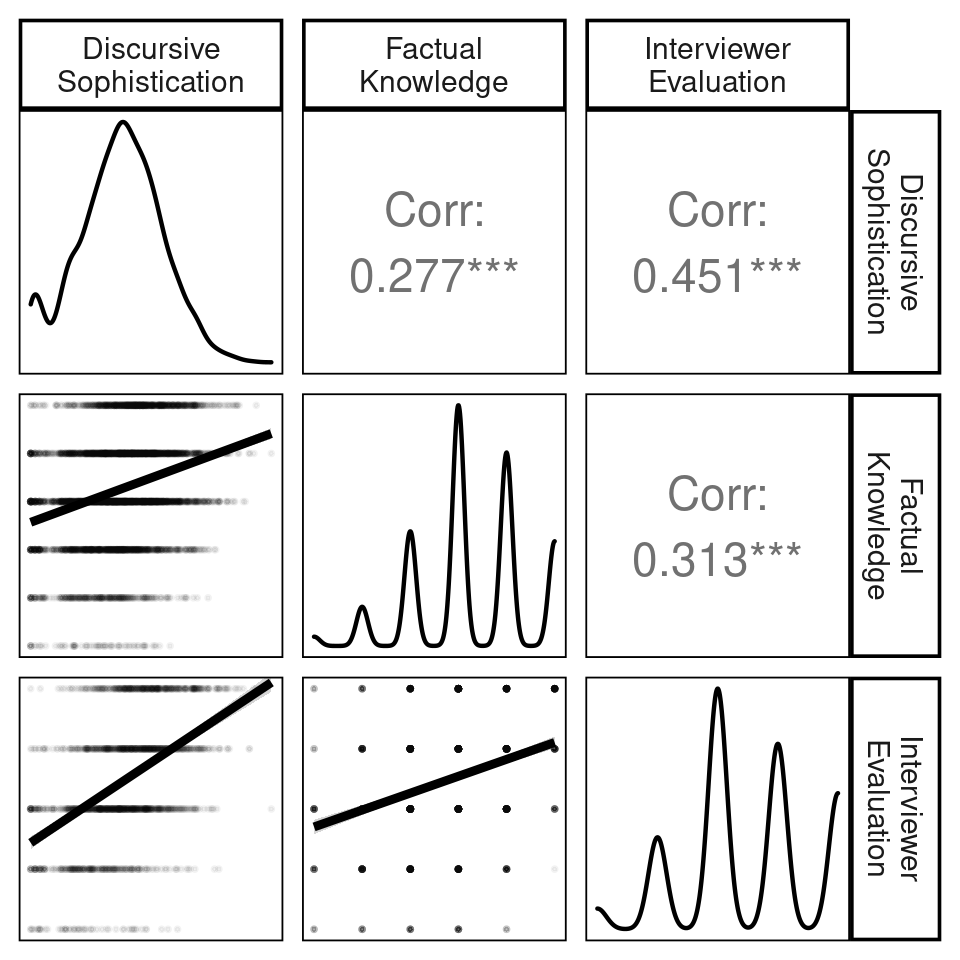
\includegraphics{/data/Dropbox/Uni/projects/2016/knowledge/fig/anes2012_corplot.png}
        \caption{2012 ANES}
    \end{subfigure}%
    \caption[Correlation matrix of discursive sophistication and conventional political knowledge metrics]{Correlation matrix of discursive sophistication and conventional political knowledge metrics. The plots on the diagonal display univariate densities for each variable. The panels in the lower triangular display the scatter plot of two measures as well as a linear fit. The upper triangular displays the correlation coefficient. All correlations reported are statistically significant with $p<.05$.}\label{fig:corplot}
\end{figure*}

\clearpage

Figure~\ref{fig:corplot} compares discursive sophistication to the conventional knowledge metrics for both waves of the ANES. Each figure presents scatterplots between individual measures (lower triangular), univariate densities (diagonal), and correlation coefficients (upper triangular). The measure of discursive sophistication is positively correlated with both conventional metrics while capturing some additional variation. Interestingly, there is a stronger correlation between discursive sophistication and interviewer evaluations than between factual knowledge and interviewer evaluations ($r=.45$ vs. $r=.31$ in 2012, and $r=.36$ vs. $r=.23$ in 2016), which indicates that the open-ended measure captures characteristics that influence subjective assessments of sophistication. Interviewers certainly form their impressions throughout the entire survey, but a respondent's verbatim answers seem to be more influential for subsequent knowledge assessments than a respondent's performance on the factual knowledge questions.

Overall, while discursive sophistication and the alternative measures are clearly correlated, the relationship between each metric is far from perfect. To provide some intuition as to whether the variation in discursive sophistication is theoretically meaningful, I present an example of open-ended responses of two individuals in the 2016 ANES who identified as Republicans and \textit{scored equally on the factual knowledge score} (3 out of 4 correct responses), but varied highly in discursive sophistication. The results are presented in Table~\ref{tab:ex1}.

\begin{table}[ht]\footnotesize\centering
\begin{tabular}{l|p{6.3cm}|p{6.3cm}}
\toprule
	& A: Low Sophistication Response & B: High Sophistication Response \\ \midrule
Clinton (+)		& 																& Politician. \\\hdashline
Clinton (-)		& The fact that she has links to Al-Qaeda. 						& Caught in lies. \\\hdashline
Trump (+)		& 																& Says what he thinks. \\\hdashline
Trump (-)		& He is going to start a civil war. I feel like he is racist. 	& Reality TV star, poor businessman \\\hdashline
Democrats (+)	& 																& Middle class minded. \\\hdashline
Democrats (-)	& 																& Too many handouts. \\\hdashline
Republicans (+)	& 																& Economic growth conscious. \\\hdashline
Republicans (-)	& 																& For the big business. \\\midrule
Disc. Soph. 	& 0.162 														& 0.461 \\\bottomrule
 \end{tabular}
\caption[Example of open-ended responses for low and high scores on discursive sophistication]{Example of open-ended responses for low and high scores on discursive sophistication with equal factual knowledge scores (3 out of 4 correct responses). Column A displays the verbatim responses of an individual who scored low on discursive sophistication and column B displays the verbatim responses of an individual who scored high on the open-ended measure. Each row represents one of the likes/dislikes items included in the analysis. Note that the responses in this table were slightly edited for readability (spelling errors removed, etc.).}\label{tab:ex1}
\end{table}

Each row in the table represents one of the open-ended responses (like/dislike for each candidate/party). Column A displays the responses of an individual who scored low on discursive sophistication and column B displays the responses of a high scoring individual. Cells are empty if a respondent refused to provide a response. Even though both individuals have the same factual knowledge score, there are systematic differences in their response behavior that can be attributed to their political sophistication. Overall, respondent A provided a less elaborate response, only focused on a narrow range of issues, and only reported attitudes on two items. Irrespective of whether one agrees with the specific statements or whether they are factually accurate (e.g., Clinton's connection to Al-Qaeda), A's response pattern is suggestive of a less sophisticated political belief system and a lower level of motivation to engage in in-depth reasoning about both parties and candidates. Overall, this initial result suggests that the variation in discursive sophistication captures meaningful differences in response behavior that overlaps with traditional knowledge metrics while displaying some unique variation. The following sections will show that this variation is also politically consequential.



\section*{Validating the Measure}
% Discursive Sophistication and Political Competence

A crucial step in validating any measure of political sophistication is to examine the extent to which it is positively related to citizen competence in modern democracies \citep{lupia2006elitism,lupia2015uninformed}. Accordingly, I consider the potential role of discursive sophistication in promoting (1) engagement and participation in politics, (2) the ability to incorporate new information, and (3) well-justified policy preferences. Each point is addressed using one of the three data sets described above.
% (5) vote choices that are consistent with underlying interests


\subsection*{Engagement and Participation in Politics}
Political sophistication is commonly expected to be strongly associated with individual engagement and participation in politics. In fact, factual knowledge items have been validated in the past based on their strong relationship with outcomes such as turnout and other forms of participation \citep[230--233]{lupia2015uninformed}. Figure~\ref{fig:knoweff} compares the effects of discursive sophistication and factual knowledge in the 2012 and 2016 ANES on four dependent variables related to political engagement: turnout, non-conventional participation, internal efficacy, and external efficacy. The model predicting turnout is estimated via logistic regression while the estimates for the three remaining dependent variables are based on OLS. Each model equation includes both sophistication measures while controlling for gender, education, income, age, race, church attendance, survey mode (face-to-face vs. online), as well as the Wordsum vocabulary score measuring verbal intelligence.\footnote{Appendix~\ref{app:variables} provides additional information on these as well as remaining variables included in subsequent analyses.}

\begin{figure}[h]\centering
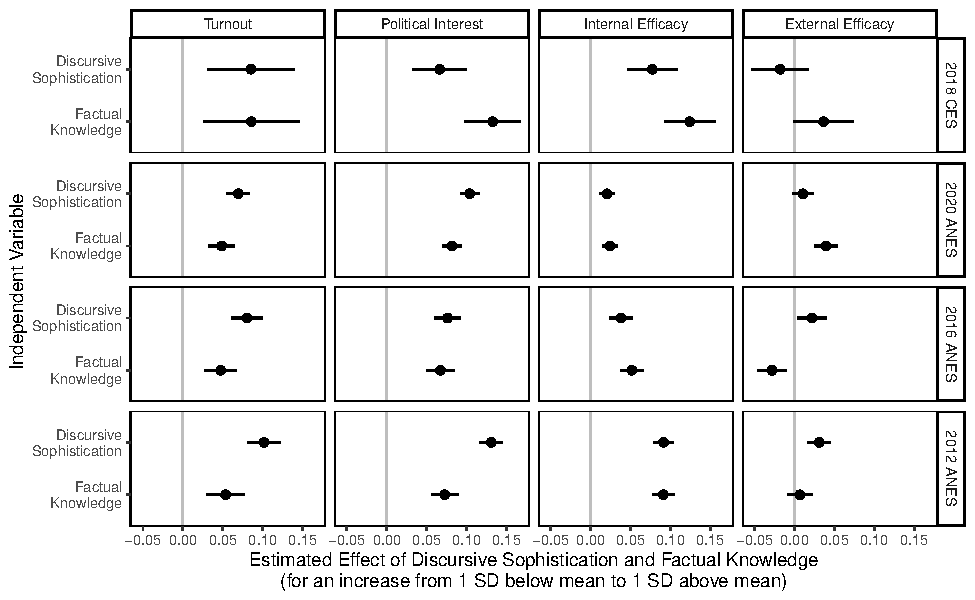
\includegraphics{/data/Dropbox/Uni/projects/2016/knowledge/fig/knoweff.pdf}
\caption[Effects of sophistication on turnout, non-conventional participation, internal efficacy, and external efficacy in the 2012 and 2016 ANES]{Effects of sophistication on turnout, non-conventional participation, internal efficacy, and external efficacy in the 2012 and 2016 ANES. For each dependent variable, the figure displays the change in expected values after increasing each sophistication measure from -1 to +1 standard deviation from its mean (including 95\% confidence intervals). Model estimates are based on logistic regression (turnout) or OLS (non-conventional participation, internal efficacy, external efficacy). Both sophistication measures are included simultaneously while controlling for gender, education, income, age, race, church attendance, survey mode, and Wordsum vocabulary scores. Full model results are displayed in the appendix, Tables~\ref{tab:knoweff2012} and \ref{tab:knoweff2016}.}\label{fig:knoweff}
\end{figure}

Each panel displays the expected difference in the respective dependent variable for a two standard deviation increase in each sophistication measure, while holding all other variables constant at their means. Overall, discursive sophistication is a stronger predictor of turnout, non-conventional participation, as well as (to a lesser extent) internal and external efficacy. In the 2012 ANES, the positive effect of factual knowledge on participation is statistically indistinguishable from zero when controlling for discursive sophistication. Furthermore, there is a negative effect of factual knowledge on external efficacy in the 2016 ANES. In contrast, the positive effect of discursive sophistication on external efficacy is more consistent with previous research. Considering these initial results, a potential concern may be that discursive sophistication is confounded by personality characteristics that influence verbatim response patterns as well as engagement. Appendix~\ref{app:personality} provides additional analyses controlling for such factors that might drive verbosity (extraversion and being reserved) as well as individual response length itself. The substantive conclusions remain unchanged.


\subsection*{Incorporation of New Information}
Competent citizens should not only engage in politics but are also expected to be sufficiently informed about the issues of the day. As such, they have to be attentive to their media environments and incorporate potentially relevant new information about parties, office-holders, and policies. Indeed, \citet{zaller1990political,zaller1992nature} and others argue that tests of factual information about politics are the best available proxy for awareness. In this analysis I draw on the 2015 YouGov study to explore whether discursive sophistication or factual knowledge serves as a better predictor of people's ability to incorporate new information from media sources. As part of the survey, respondents were asked to read a newspaper article about a fictional infectious disease and were subsequently asked to answer questions about information provided in the article (e.g. regarding symptoms, modes of contraction etc.). I compute an additive index counting the pieces of information that were correctly recalled (\textit{information retrieval}) as a measure of the ability to retrieve information from a news article on a non-partisan issue that is related to public health policies. 

\begin{figure}[h]\centering
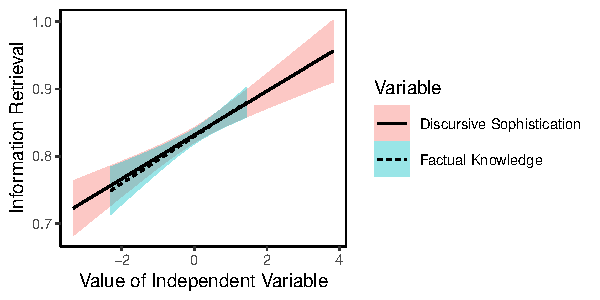
\includegraphics{/data/Dropbox/Uni/projects/2016/knowledge/fig/yg_disease.pdf}
\caption[Expected information retrieval in the 2015 YouGov Study as a function of political sophistication]{Expected information retrieval in the 2015 YouGov Study as a function of political sophistication (including 95\% confidence intervals). Estimates are based on a linear regression model controlling for education, income, age, church attendance, gender, and race. Full model results are displayed in the appendix, Table~\ref{tab:yg_disease}.}\label{fig:yg_disease}
\end{figure}

Figure~\ref{fig:yg_disease} displays the relationship between political sophistication and disease information retrieval in the 2015 YouGov study. Estimates are based on a linear regression model controlling for education, income, age, church attendance, gender, and race. As a benchmark for discursive sophistication, I again consider the effect of factual knowledge based on a battery of eight items similar to the knowledge questions in the ANES. Both discursive sophistication as well as factual knowledge increase the amount of information individuals are able to recall from a news article discussing a fictional disease. Similar to the previous results, the effects are stronger for discursive sophistication than for factual knowledge scores. The degree to which citizens discuss their own political beliefs in a more elaborate manner is not only a stronger predictor of political engagement but also serves as a better proxy for the ability to incorporate new information about a non-partisan issue.


\subsection*{Well-Justified Policy Preferences}
Beyond the ability to incorporate new information, competent citizens should be knowledgeable about the underlying policies themselves and be able to justify their own preferences. Here, I explore the extent to which high levels of discursive sophistication correspond to well-justified policy preferences in open-ended responses. As mentioned above, the Swiss surveys included items that asked respondents to explain why they voted in favor or against a given proposition in multiple policy referenda. To corroborate the face validity of discursive sophistication, I examine whether the measure is related to Colombo's \citeyearpar{colombo2016justifications} manual coding of the respondents' \textit{level of justification}, which assessed the content, elaboration, and complexity of open-ended responses.

The results are presented in Figure~\ref{fig:swiss_ggridges}, which displays the distribution of discursive sophistication for each level of justification coded by \citet{colombo2016justifications} as well as the correlation coefficients for both respective variables. Across all three language groups, discursive sophistication is systematically higher among respondents with the highest level of justification and both measures are positively correlated ($r=0.26, 0.30$, and $0.35$, respectively). The proposed measure of discursive sophistication therefore shows a high degree of correspondence with individual levels of justification assessed by independent manual coders.

\begin{figure}[h]\centering
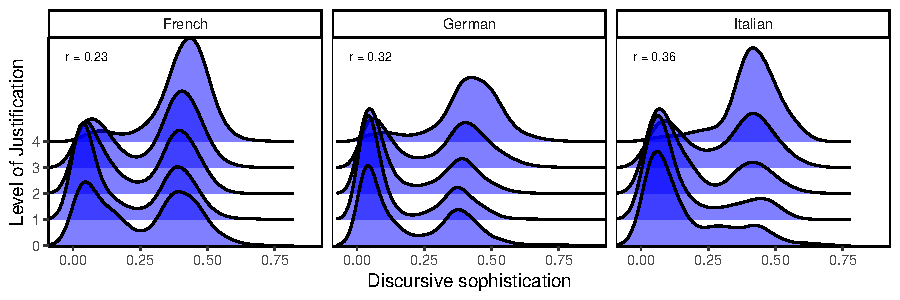
\includegraphics[scale=1]{/data/Dropbox/Uni/projects/2016/knowledge/fig/swiss_ggridges.pdf}
\caption[Discursive sophistication and manually coded level of justification in Swiss post-referendum surveys]{Discursive sophistication and manually coded level of justification \citep{colombo2016justifications} in Swiss post-referendum surveys. The plot compares kernel densities of discursive sophistication for each manually coded level of justification.}\label{fig:swiss_ggridges}
\end{figure}

To summarize, the results presented thus far indicate that discursive sophistication shares common characteristics with factual political knowledge measures. Compared to conventional metrics, the proposed measure performs at least as well as a predictor of essential competences that allow citizens to engage successfully in politics. In fact, discursive sophistication is a stronger predictor of certain outcomes (such as different forms of political participation) than conventional knowledge scores. In the following, I turn to an application to illustrate how discursive sophistication can help refine important previous insights from the literature on political knowledge.

%\clearpage
\section*{Reassessing the Gender Gap}
How do women and men compare on the different metrics of political sophistication in the surveys analyzed in the present study? The top row of Figure~\ref{fig:meandiff} displays the average levels of discursive sophistication as well as conventional metrics comparing both genders. While we observe a sizable and statistically significant gender gap for factual knowledge in both ANES surveys, this difference disappears for discursive sophistication. These results are replicated in the 2015 YouGov survey. Even though women do not perform as well as men on political quizzes, they do not differ substantially in complexity and sophistication when describing their political preferences.

\begin{figure}[h]\centering
	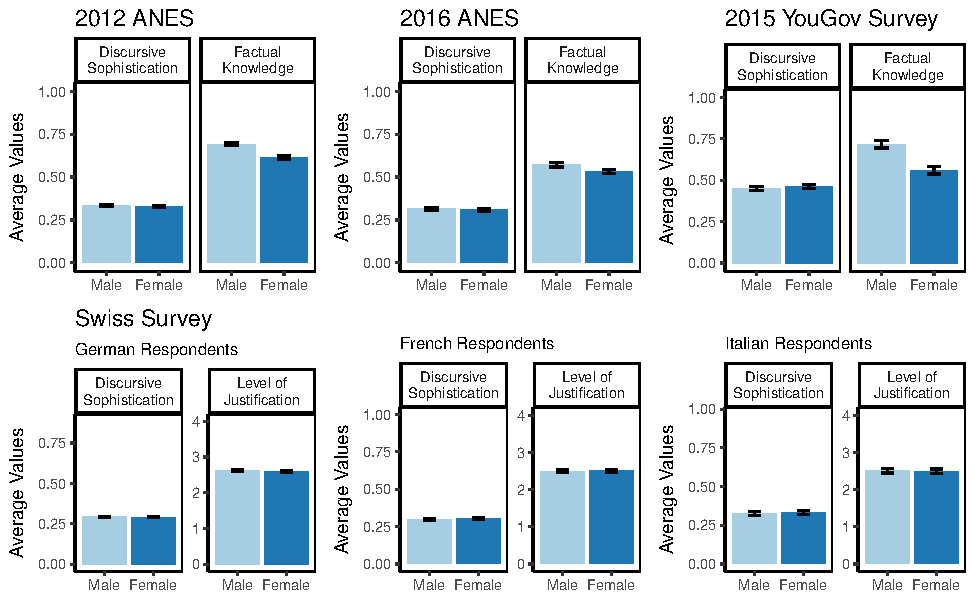
\includegraphics{/data/Dropbox/Uni/projects/2016/knowledge/fig/meandiff.pdf}
	\caption[The gender gap in political sophistication]{The gender gap in political sophistication. The figures display mean levels of sophistication for each measure comparing women and men (including 95\% confidence intervals). Gender differences in factual knowledge in the 2012/2016 ANES and 2015 YouGov survey (top row) are statistically significant with $p<.05$. Gender differences in discursive sophistication and manually coded levels of justification \citep{colombo2016justifications} are not statistically significant.}\label{fig:meandiff}
\end{figure}

\clearpage

Of course, we need to make sure that this absence of a gender gap in discursive sophistication is not idiosyncratic to the particular measurement approach proposed here. One way to investigate this question is to examine gender differences in discursive sophistication using data from \citet{colombo2016justifications} and comparing them to her manually coded measure. That way, we can not only determine whether the lack of a gender gap in discursive sophistication replicates in the third survey, but also check whether there is an equivalent lack of gender differences in Colombo's alternative measure of citizen competence in direct democracies. If discursive sophistication captures a person's motivation to undertake in-depth reasoning and form quality opinions (and assuming these characteristics do not differ by gender), there should be no difference between women and men on either metric (discursive sophistication and Colombo's measure). As shown in the bottom row of Figure~\ref{fig:meandiff} there are indeed no significant gender differences on \textit{both} metrics across all three languages in the Swiss referendum surveys. The absence of a gender gap is consistent whether open-ended responses are coded manually or using the proposed measure of discursive sophistication.

Next, we have to consider whether the apparent gender gap in factual knowledge is a manifestation of real differences between women and men. Prior research attributes at least part of the gap to actual discrepancies in individual resources and engagement. Accordingly, we need to control for these determinants of political knowledge to provide a more comprehensive examination of the veracity of observed gender differences. Figure~\ref{fig:determinants} displays estimated effects of various potential common determinants of factual knowledge and discursive sophistication on both measures. Previous studies consistently showed that political information levels are positively related to high media exposure, frequent political discussions, education, and income. Furthermore, I include age, race, church attendance, and survey mode (face-to-face vs. online) as additional control variables.

\begin{figure}[h]\centering
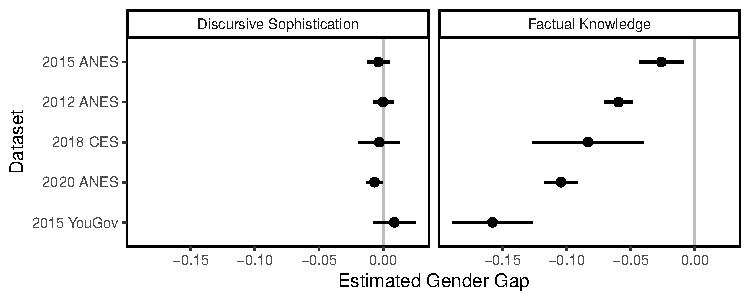
\includegraphics{/data/Dropbox/Uni/projects/2016/knowledge/fig/determinants.pdf}
\caption[Common determinants of political sophistication]{Common determinants of political sophistication. Estimates are OLS regression coefficients with 95\% confidence intervals. Dependent variables are discursive sophistication as well as factual political knowledge. Full model results are displayed in the appendix, Tables~\ref{tab:determinants_anes} and \ref{tab:determinants_yg}.}\label{fig:determinants}
\end{figure}

After controlling for common determinants, discursive sophistication again reveals no significant differences between women and men in both ANES surveys as well as the 2015 YouGov study. The gender gap in factual political knowledge, however, persists and is substantively as well as statistically significant. Thus, a considerable portion of the observed differences in factual knowledge between women and men cannot attributed to underlying disparities in resource-related factors or engagement. It is worth pointing out in this context, that the effects of the control variables are quite similar across both measures and different surveys. Knowledge and discursive sophistication are significantly higher among respondents who are more exposed to political news media, discuss politics frequently, are more educated, and have higher income.\footnote{An interesting deviation, however, is the effect of survey mode in the 2012 and 2016 ANES. Respondents in online surveys score significantly higher on factual knowledge than in face-to-face interviews. This difference can be attributed to the fact that individuals are able to look up answers for factual knowledge questions while taking an online survey \citep[cf.][]{clifford2016cheating}. For discursive sophistication, on the other hand, individuals perform better in the face-to-face survey. Open-ended answers in online surveys may be less elaborate because respondents have to manually type their responses.} Overall, the finding that determinants of political sophistication are consistent across models lends additional validity to the open-ended measure.


\section*{Explaining the (Lack of a) Gender Gap}

% Summarizing the results thus far, there is no evidence for systematic differences between women and men in discursive sophistication.
In summary, the analyses only reveal a significant gender gap based on conventional recall-based measures of political knowledge, a result that previous research attributed---at least partly---to the format (e.g., availability of ``Don't Know'' options) and content (e.g., focusing on issues that are less relevant to women) of the question batteries. This section explores whether these arguments provide a sufficient explanation for the conflicting results for discursive sophistication---namely the complete lack of systematic differences between women and men. In other words, is it the \textit{existence} of a gender gap in factual knowledge or the \textit{absence} of a gap in discursive sophistication, that is more likely to be an artifact of the respective measurement approach?

The first set of arguments about why conventional metrics may overstate potential gender differences is based on the finding that women are less likely to guess than men \citep{mondak2004knowledge}. Arguably, respondents' differential willingness to admit not knowing the answer to a question is certainly less of an issue when they are simply asked to voice their opinions rather than being quizzed on political facts. Following best practices, however, both waves of the ANES as well as the YouGov study omitted ``Don't Know'' options in their recall questions. Differential propensity to guess can therefore not be viewed as a valid explanation for the gender gap in factual knowledge observed here. At the same time, the lack of significant differences between women and men in discursive sophistication may itself be the product of selection biases in women's willingness to answer open-ended question in the first place. Following this argument, it could be the case that only women who are highly sophisticated provide a response, thereby misleadingly closing the gender gap in the discursive measure. There are two reasons why that is unlikely to be the case. First, as the analyses have shown, this proposed selection mechanism does not diminish gender differences in factual knowledge. Second, and more importantly, there are no significant differences between men's and women's willingness to answer open-ended questions (ANES 2012: $z = 1.630$, $p = 0.103$; ANES 2016: $z = 0.464$, $p = 0.643$). In fact, adjusting for potential selection effects when examining determinants of sophistication does not change the substantive conclusions presented in the discussion of Figure~\ref{fig:determinants}.

The second major explanation for the gender gap in political knowledge focuses on the question content. At the outset of this paper, I discussed how \citet{cramer2017fact}, along with other scholars, criticized traditional knowledge batteries for focusing erroneously on what people do not know. By choosing a specific set of recall questions as a general metric for political knowledge, researchers are making strong assumptions about the information deemed necessary for competent decision-making. As it turns out, these item batteries usually focus on male-dominated topics in politics \citep{dolan2011women}. Open-ended questions, on the other hand, make it possible to directly study the information that is in fact available to citizens and---importantly---to examine how they apply their knowledge when discussing their political preferences.

Accordingly, if it is the case that the gender gap in discursive sophistication is nonexistent simply because open-ended questions allow women to raise political considerations particularly salient to them, then we should be able to observe systematic variation in types of issues discussed by women and men, respectively. Luckily, we can directly examine such gender differences in topic prevalence within the structural topic model framework used to measure discursive sophistication. More specifically, gender is included in the model as one of the covariates that influences how often each topic is discussed by a respondent \citep[see also][for details]{roberts2014structural}.

\begin{figure}[h]\centering
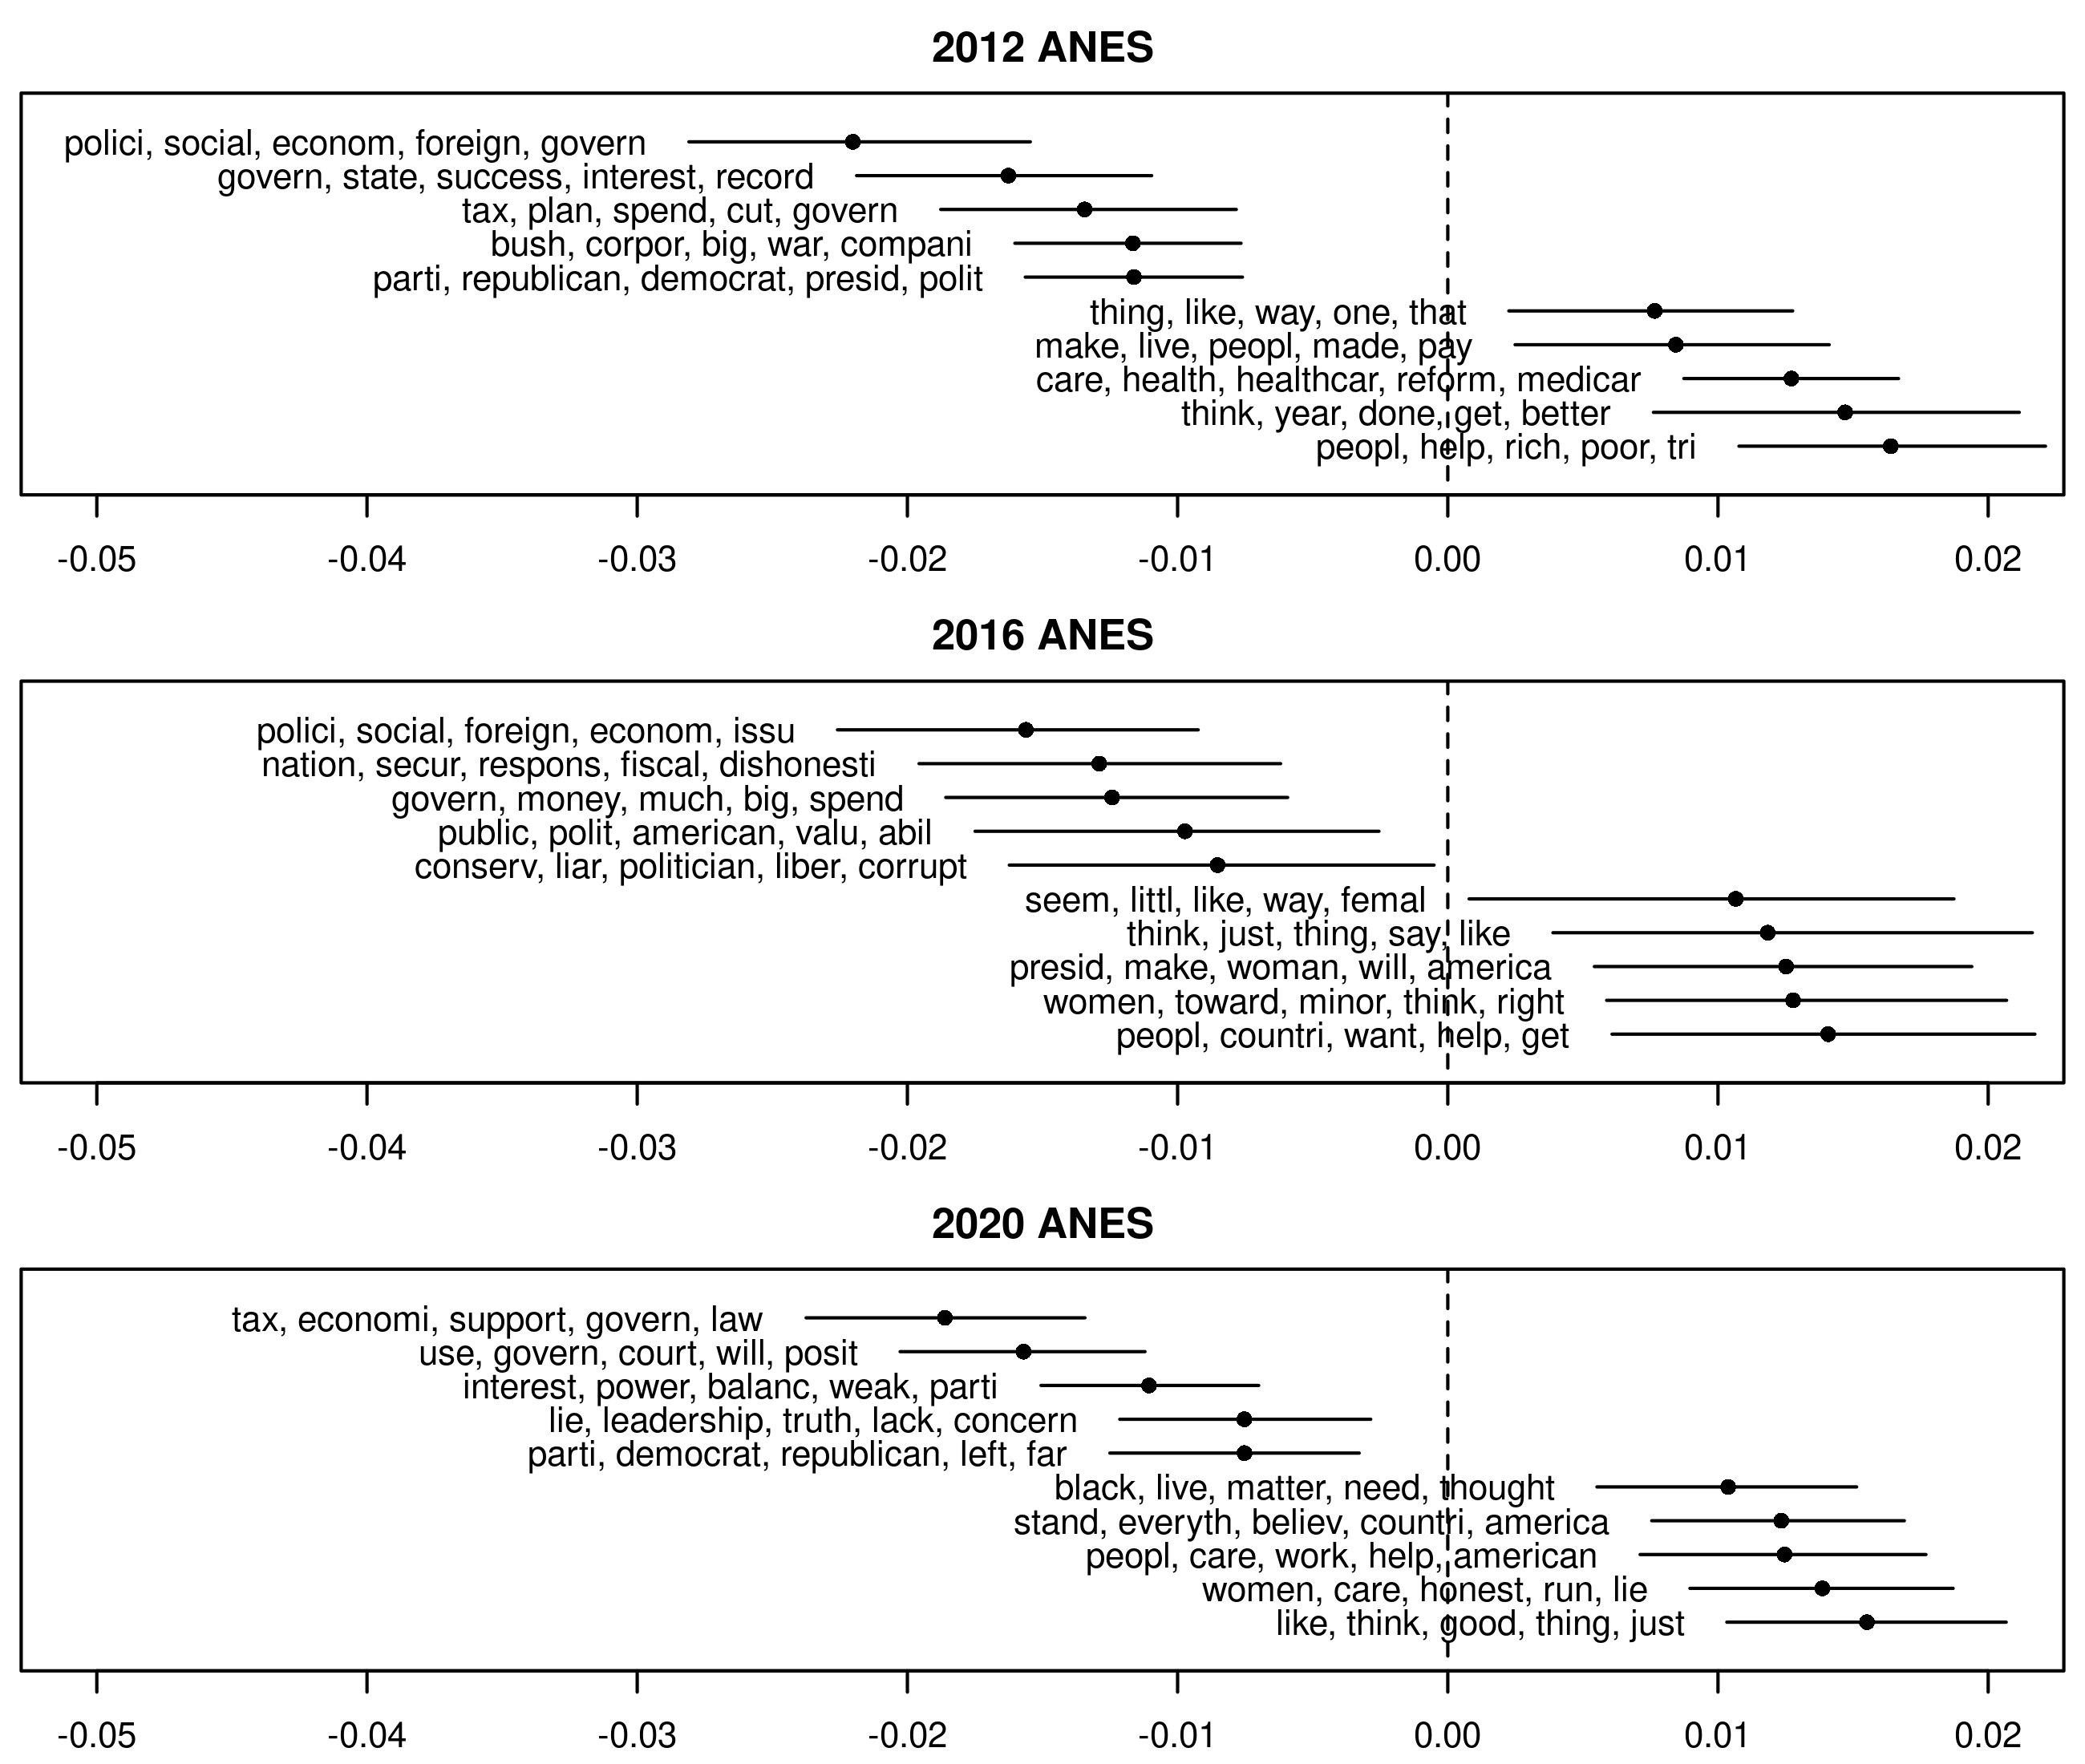
\includegraphics[width=.9\textwidth]{/data/Dropbox/Uni/projects/2016/knowledge/fig/stm_gender.png}
\caption[Gender differences in topic proprtions in open-ended responses]{Gender differences in topic proportions in open-ended responses based on the structural topic model used to compute discursive sophistication (including 95\% confidence intervals). Coefficients indicate the difference in predicted topic prevalence among women and men; positive values indicate higher prevalence among women. Labels are based on the five highest probability terms related to the topic.
%Full model results are displayed in the appendix, Table~\ref{tab:determinants}
}\label{fig:stm_gender}
\end{figure}

\clearpage

In this last analysis, I therefore explore how women and men differ in topical prevalence across open-ended responses in the 2012 and 2016 ANES. Figure~\ref{fig:stm_gender} displays the subset of topics that shows the largest absolute gender difference in topic prevalence in both waves. Positive coefficients indicate that women are more likely than men to mention a given topic, and vice versa. As such, the top six topics are more prevalent among men and the bottom six are more likely to be mentioned by women. The label for each coefficient consists of the five highest probability terms related to the topic in order to illustrate its content.

Taking the 2012 ANES as an example, the topic consisting of terms such as \textit{right}, \textit{women}, and \textit{equal} is significantly more likely to be mentioned by women. On the other hand, men are more likely to mention the topic revolving around terms like \textit{budget}, \textit{balance}, and \textit{privat}. Overall, across both waves of the ANES, women were less likely than men to discuss foreign affairs, economic issues, or the Supreme Court. Instead, they focused on issues related to women's rights, equality, and health care. The considerations raised by women when discussing their political preferences are therefore clearly different from men's and---crucially---the issues discussed by men happen to be more aligned with the type of questions usually covered in standard political knowledge batteries (i.e., pertaining to the economy, institutions, elites, etc.). For example, men are more likely to mention considerations related to the federal budget in their open-ended responses. At the same time, two of the five knowledge questions included in the 2012 ANES pertain to government spending: one asking respondents to compare the federal deficit to levels in 1990, the other requiring a comparison of federal spending on different programs such as foreign aid, medicare, and national defense.

Overall, the results indicate that gender differences in conventional knowledge metrics can at least partly be explained by the fact that the issues women care about are not represented in standard item batteries. When using the alternative measure---discursive sophistication---any evidence for systematic differences between women and men disappears since open-ended questions about political preferences allow respondents to focus on different issues. 

% TODO: Make a connection back to Druckman here?


\section*{Discussion and Conclusion}
% What is a competent citizen? One who has good reasons for his or her attitudes... we can measure that when examining how repondents talk about their political beliefs.

% 1) Repeat general argument
Political scientists should worry less about pure levels of \textit{factual knowledge} and instead focus on the necessary conditions for individuals to make \textit{competent} decisions. Competence in elections, for example, requires citizens to hold informed attitudes about their representatives. Factual knowledge about political institutions might be a useful proxy in certain scenarios, but it cannot address directly whether individuals hold well-considered opinions about political actors they try to hold accountable. In comparison, the measure of discursive sophistication proposed here is agnostic about the specific contents of people's beliefs, but directly targets the complexity of expressed attitudes related to the political task. It can therefore be easily applied to assess sophistication in any decision-making context (such as policy referenda or local elections) by fielding targeted open-ended questions related to the relevant underlying beliefs and preferences.

% 2) Summarize main findings of the paper
The findings presented in this paper show that conventional knowledge indices and the open-ended measure share a substantial amount of variance. However, they are far from being identical and capture different aspects of sophistication. In fact, discursive sophistication is a stronger predictor of political engagement and efficacy than traditional metrics. It is also strongly related to people's ability to incorporate new information from news sources and shows a high degree of overlap with manually coded levels of justification. Most importantly, using the discursive measure, any evidence for the gender gap commonly reported using factual knowledge scales disappears. Women might know fewer facts about political institutions, but they do not differ substantively in the complexity of their expressed political beliefs. The fact that women perform just as well as men on discursive sophistication across various surveys can be attributed to the fact that they focus on different considerations when evaluating political parties and candidates.

% 3) Discuss implications for competence and tie back to Druckman's argument
From a normative perspective, there is no reason to assume that a particular set of issues should be more important for citizens' preference formation or competence in elections. Whether one cares more about the federal budget or reproductive rights, the most important question is whether citizens think deeply about the issues they care about and incorporate them accordingly when making their vote choices. As \citet{druckman2014pathologies} argues, citizen competence (for example in elections) should not be evaluated based on their ability to recall unrelated facts about political institutions, but rather focus people's motivation to form quality opinions---which implies that they focus on the issues most important to them. As it turns out, while the types of issues raised women and men differ systematically, there is no reason to assume that women are therefore less sophisticated or competent in the realm of politics.

% 4) Discuss how discursive sophistication can be used to improve knowledge batteries
This issue has been recognized in the literature before \citep[e.g.,][]{graber2001processing,dolan2011women}, but it cannot be properly addressed while relying exclusively on off-the-shelf recall questions to measure political knowledge. What is more, there is thus far no principled approach to develop new sets of items that focus less on male-dominated issues. Beyond proposing an alternative measurement approach, the framework presented in this paper can help provide such a first step towards devising balanced recall items. More specifically, examining the types of issues women and men emphasize when discussing their political preferences can serve as a guide to select new sets of knowledge questions. Granted, more research is necessary to explore whether factual knowledge questions selected based on open-ended responses are indeed more balanced with regard to gender differences. To the extent that this indeed proves to be a useful heuristic for item selection, researchers planning a survey could rely on pilot studies fielding open-ended questions in order to devise balanced factual knowledge items in the main survey.

% 5) Mention potential drawbacks and disadvantages
That being said, relying on open-ended responses to assess political sophistication also comes with potential drawbacks. First and foremost, elaboration in verbatim attitude expression may be more prone to biases due to differential levels of motivation to answer survey questions. It should be noted, however, that conventional knowledge metrics are not free from survey effort effects either---as indicated for example by the fact that scores can be improved by providing monetary incentives for correct responses \citep{prior2008money}---and future studies should investigate the extent to which discursive sophistication is subject to similar deviations. A related potential confounding factor that is unique to open-ended responses is the respondents' general linguistic skills or verbal verbosity, which may again influence elaboration in open-ended responses but is orthogonal to political sophistication.

% 6) Discuss why the issues are probably not that bad
One reason why these potential drawbacks may be less worrisome is that the proportion of respondents who refuse to answer any open-ended question in the first place is very low, which indicates that people are sufficiently motivated to engage with the survey. Furthermore, controlling for pure response length did not change the substantive conclusions regarding the effects of discursive sophistication on, for example, political participation or efficacy. The results were also robust for the inclusion of measures of linguistic skills or personality characteristics like extraversion. In a similar vein, the gender gap finding did not appear to be driven by selection effects, which again suggests that survey effort---albeit an important confounding factor to consider---is unlikely to jeopardize the substantive conclusions presented in this paper.

% 7) Bring up survey mode, discuss advantage regarding cheating
Nevertheless, it is important to keep in mind the differential role of survey mode when comparing factual knowledge and discursive sophistication. Open-ended responses in face-to-face or phone interviews are relatively effortless since they are not unlike voicing your opinion in regular conversations and do not require respondents to transform their thoughts into fixed response categories \citep[e.g.,][]{sudman1996thinking}. Unsurprisingly though, respondents tend to provide less elaborate responses in online surveys, resulting in systematically lower discursive sophistication scores (see Figure~\ref{fig:determinants}). Knowledge quizzes conducted online, on the other hand, are prone to bias in the opposite direction due to respondents' tendency to cheat by looking up correct answers \citep{clifford2016cheating}. Ultimately, more work is needed to explore how survey mode affects discursive sophistication and factual knowledge scores, especially focusing on ways to reduce the effort in answering open-ended questions in online surveys.

% 8) Manual coding as an alternative to overcome these issues?
Lastly, even if one supports the general notion that open-ended responses can provide useful insights, a skeptic may still argue that manual coding is preferable to the automated framework presented here. However, manual coding of open-ended responses is not always feasible in the context of large-scale surveys, since it can be labor-intensive and requires extensive contextual knowledge such as high levels of language proficiency. The Swiss surveys in Colombo's \citeyearpar{colombo2016justifications} study, for example, were conducted in three different languages (German, French, and Italian) and ranged across numerous policy referenda. More importantly, knowledge assessments can be biased by the level of political agreement between individuals \citep[e.g.,][]{ryan2011accuracy}. The measurement approach presented here, on the other hand, is easily replicable and reproducible, is not affected by subjective judgments, and can be directly applied to large-scale surveys in multiple contexts across different languages.

% 9) BIG CONCLUSION: clearly state that it is not to be viewed as a replacement but rather a substitute for political knowledge questions
In the past, scholars have argued that testing for factual information, despite its shortcomings, still provides the best available measure of political awareness as it captures ``what has actually gotten into people's minds, which, in turn, is critical for intellectual engagement with politics'' \citet[21]{zaller1992nature}. The results presented in this paper suggest that a direct examination of open-ended responses provides a viable supplemental approach that promises new insights into how people make up their mind about politics.

